% Unofficial University of Cambridge Poster Template
% https://github.com/andiac/gemini-cam
% a fork of https://github.com/anishathalye/gemini
% also refer to https://github.com/k4rtik/uchicago-poster

\documentclass[final]{beamer}

% ====================
% Packages
% ====================

\usepackage[T1]{fontenc}
\usepackage{lmodern}
\usepackage[size=a1,scale=1.0]{beamerposter}
\usetheme{gemini}
\usecolortheme{cam}
\definecolor{junglegreen}{RGB}{41,171,135}
\definecolor{darkjungle}{RGB}{0, 102, 68}
\setbeamercolor{headline}{bg=junglegreen}
\usepackage{graphicx}
\usepackage{booktabs}
\usepackage[numbers]{natbib}
\usepackage{tikz}
\usepackage{pgfplots}
\usepgfplotslibrary{external}
\pgfplotsset{compat=1.18}
\usepackage{anyfontsize}

% ====================
% Lengths
% ====================

% If you have N columns, choose \sepwidth and \colwidth such that
% (N+1)*\sepwidth + N*\colwidth = \paperwidth
\newlength{\sepwidth}
\newlength{\colwidth}
\setlength{\sepwidth}{0.025\paperwidth}
\setlength{\colwidth}{0.3\paperwidth}

\newcommand{\separatorcolumn}{\begin{column}{\sepwidth}\end{column}}

% ====================
% Title
% ====================

\title{Anakondaen}

\author{Sabine Christoffersen \inst{} \and Jannik Busse Guldmand \inst{}}

\institute[shortinst]{\inst{} Data Science - DS805 Multivariat statistisk analyse}

% ====================
% Footer (optional)
% ====================

\footercontent{
  Anaconda Data, Table 6.19, s.357 i bogen Applied Multivariate Statistical Analysis \hfill
  \hfill
  \href{https://github.com/guldmand/DS805_Multivariat_Poster}{\texttt{github.com/guldmand/DS805\_Multivariat\_Poster}}
}
% (can be left out to remove footer)

% ====================
% Logo (optional)
% ====================

% use this to include logos on the left and/or right side of the header:
% \logoright{\includegraphics[height=7cm]{logo1.pdf}}
% \logoleft{\includegraphics[height=7cm]{logo2.pdf}}

% ====================
% Body
% ====================

\begin{document}

% Force block heading to the left
\makeatletter

% Force non bold heading


% Force junglegreen block heading
\setbeamercolor{block title}{fg=junglegreen}

\setbeamertemplate{block begin}{
  \par\vskip\medskipamount
  \begin{beamercolorbox}[colsep*=.75ex]{block title}
    \usebeamerfont*{block title}
    \raggedright\insertblocktitle
  \end{beamercolorbox}
  {\parskip0pt\par}
  % Add horizontal rule
  \nointerlineskip
  \hspace*{0pt}\rule{\linewidth}{0.4pt}
  \vskip0.5ex
  \usebeamerfont{block body}
  \begin{beamercolorbox}[colsep*=.75ex,vmode]{block body}
    \ignorespaces
}

% Refer to https://github.com/k4rtik/uchicago-poster
% logo: https://www.cam.ac.uk/brand-resources/about-the-logo/logo-downloads
\addtobeamertemplate{headline}{}
{
  \begin{tikzpicture}[remember picture,overlay]
  
    % SDU logo (venstre side)
    \node[anchor=north west, xshift=1cm, yshift=-0.2cm] 
      at (current page.north west) 
      {
\includegraphics[height=5cm]{logos/SDU.png}};

	 % Snake logo (højre side)
    \node[anchor=north east, xshift=-1cm, yshift=3.5cm] 
      at (current page.north east) 
      {
\includegraphics[width=12cm, angle=180]{logos/snake_white.png}};


  \end{tikzpicture}
}

\begin{frame}[t]
\begin{columns}[t]
\separatorcolumn

\begin{column}{\colwidth}

  \begin{block}{Introduktion}
  \justifying

	\textbf{Anakondaen} (\textit{Eunectes murinus}), også kendt som
	den grønne anakonda, er én af verdens største og
	tungeste slanger. Den hører til kvælerslangerne
	og lever primært i tropiske og fugtige områder i
	Sydamerika – især i Amazonasflodens vandrige
	lavlandsområder.
	\vspace{0.5em}
	
	
	\begin{columns}
	
	  % Højre kolonne: Start på teksten (første 2-3 linjer)
  \begin{column}{0.40\textwidth}

  Anakondaen er semi-akvatisk og tilbringer
	størstedelen af sin tid i vand, hvor dens store
	masse ikke begrænser dens bevægelighed. I vandet
	jager den fisk, fugle, kapivarer og endda
	kaimaner. Den dræber sit bytte ved at kvæle det
	med sin stærke muskulatur.
	\vspace{1em}

	I dette projekt undersøger vi forskelle i længde
	og vægt mellem hunner og hanner, baseret på data
	fra 56 individer. Formålet er at analysere om
	køn har en signifikant effekt på anakondaens
	fysiske egenskaber ved brug af multivariate
	statistiske metoder.

  \end{column}
  
    % Venstre kolonne: Billedet
  \begin{column}{0.55\textwidth}
    \begin{figure}
      \centering
      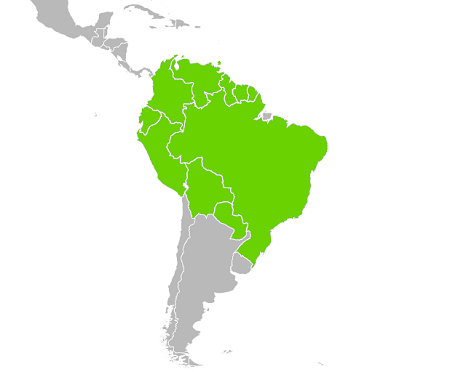
\includegraphics[width=0.9\linewidth]{logos/habitat.png}
      \vspace{1.0em}
      
      \textbf{\textcolor{junglegreen}{Figur 1:}} Anakondaens habitat
    \end{figure}
  \end{column}



  
\end{columns}
	
  \end{block}
  
  
\vspace{-1em}
\begin{block}{Datasæt}
\justifying

Anakonda-datasættet består af \textbf{56 observationer} og \textbf{3 variable}:
%Anakonda-datasættet består af \strong{56 observationer} og \strong{3 variable}


\begin{itemize}
	\item \textbf{Snude vent længde (cm)} — længden fra snude til den bageste åbning  (numerisk)
	\item \textbf{Vægt (kg)} — anakondaens vægt i kilo (numerisk)
	\item \textbf{Køn} - køn som kategorisk variabel med værdierne \textit{Hun} og \textit{Han} (faktor)
\end{itemize}

Datasættet stammer fra \textit{Table 6.19} i bogen \textit{Applied Multivariate Statistical Analysis} (6. udgave) og udgør grundlaget for vores analyse. Variablerne repræsenterer nøgleegenskaber ved anakondaer og muliggør en direkte sammenligning af længde og vægt mellem kønnene.

\vspace{1em}

De to numeriske variable indgår som responser i de multivariate analyser, mens køn anvendes som gruppering til at identificere kønsforskelle.

	\begin{figure}[h!]
	\centering
	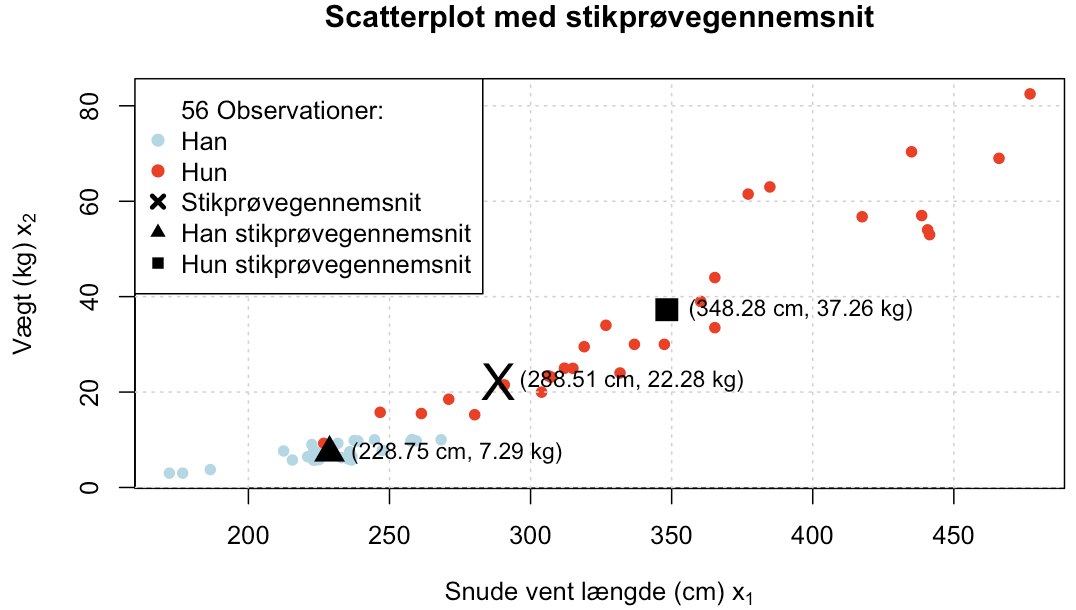
\includegraphics[width=0.80\linewidth]{plots/scatter_final5.png}
	
	\textbf{\textcolor{junglegreen}{Figur 2:}} Scatterplot fordelt på køn
	
	
	\end{figure}

\end{block}

  \vspace{-2em}
  \begin{block}{Normalitetstest}
    \justifying

    \begin{figure}[h!]
	\centering
	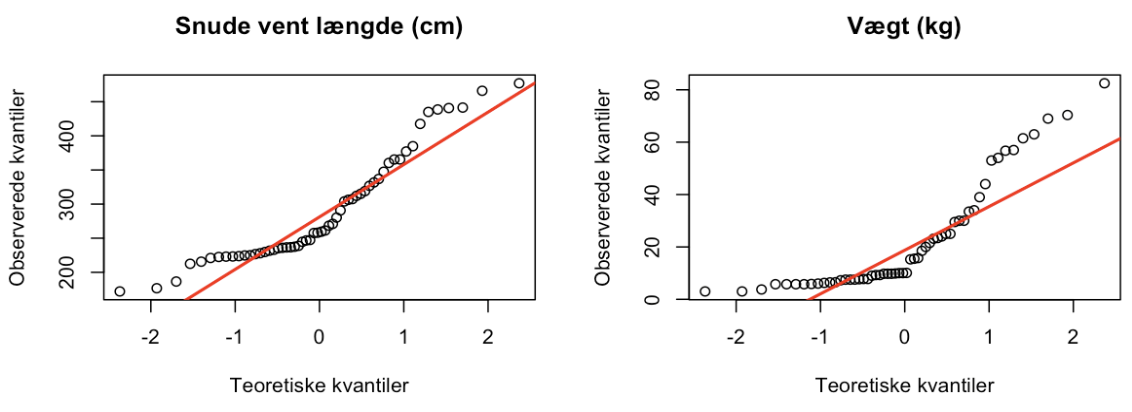
\includegraphics[width=0.95\linewidth]{plots/qq_1final.png}

	\end{figure}
	
  \end{block}

\end{column}

\separatorcolumn


\begin{column}{\colwidth}
\justifying

\begin{figure}[h!]
	\centering
	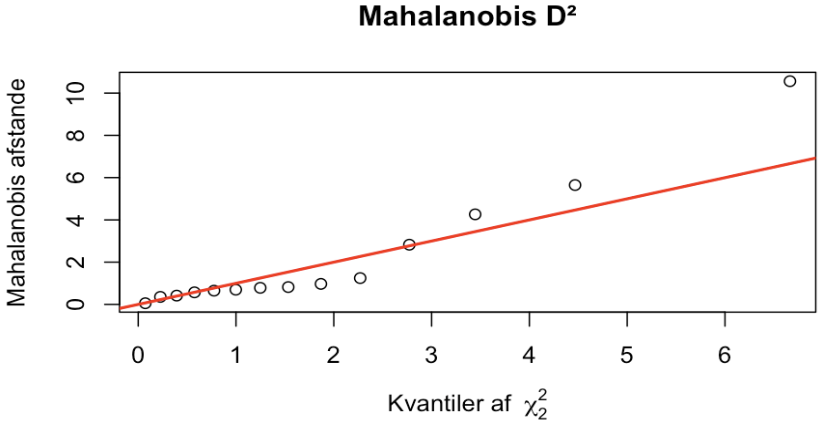
\includegraphics[width=0.75\linewidth]{plots/qq_3.png}

	\textbf{\textcolor{junglegreen}{Figur 3:}} Q-Q Plots 	
\end{figure}

De univariate (marginale) og det multivariate Q-Q plot indikerer, at anakonda-dataene ikke følger en normalfordeling.
\vspace{1em}

Vi tester for univariat normalfordelt data, da dette er en forudsætning for at udføre univariat-inferens (T-test). Vi tester for multivariat normalitet, da dette er en forudsætning for at udføre multivariat inferens.

\vspace{0.5em}


  
\begin{block}{Univariat inferens (T-tests)}
  \justifying

 Vi har udført to uafhængige T-tests for at undersøge, om der er forskelle i \textbf{Snude vent længde (cm)} og \textbf{Vægt (kg)} mellem han- og hun-anakondaer.
	
I de univariate T-tests tester vi om 
%\( \boldsymbol{\mu}_{\text{Hun}} = \boldsymbol{\mu}_{\text{Han}}: \)
\textbf{\boldmath$\boldsymbol{\mu}_{\text{Hun}} = \boldsymbol{\mu}_{\text{Han}}$}



\begin{itemize}
  \item $H_0$: Der er ingen forskel i gennemsnitlig Snude vent længde mellem kønnene.
  \item $H_1$: Der er forskel i gennemsnitlig Snude vent længde mellem kønnene.
  
  \vspace{0.5em}
  
  \item $H_0$: Der er ingen forskel i gennemsnitlig vægt mellem kønnene.
  \item $H_1$: Der er forskel i gennemsnitlig vægt mellem kønnene.
\end{itemize}
\vspace{1em}
	
	\vspace{-1em}
	
  \begin{table}
    \centering
    %\begin{tabular}{l r r r r l}
    %  \toprule
    %  \textbf{Variabel} & \mu\textbf{Hun} & \mu\textbf{Han} & \textbf{T-værdi} & \textbf{P-værdi} & \textbf{95\% CI} \\
    %  \midrule
    %  Snude vent længde (cm) & 348.28 & 228.75 & 8.76 & $< 5.98\cdot10^{-12}$ & [92.17, 146.88] \\
    %  Vægt (kg)       & 37.26  & 7.29   & 7.85 & $< 1.74\cdot10^{-10}$ & [22.32, 37.63] \\
    %  \bottomrule
    % \end{tabular}
    
  \begin{tabular}{l r r r r l}
  \toprule
  \textbf{Variabel} & \textbf{$\boldsymbol{\mu}_{\mathrm{Hun}}$}
 & \textbf{$\boldsymbol{\mu}_{\mathrm{Han}}$} & \textbf{T-værdi} & \textbf{P-værdi} & \textbf{95\% KI} \\
  \midrule
  Snude vent længde (cm) & 348.28 & 228.75 & 8.76 & $< 5.98\cdot 10^{-12}$ & [92.17, 146.88] \\
  Vægt (kg) & 37.26 & 7.29 & 7.85 & $< 1.74\cdot 10^{-10}$ & [22.32, 37.63] \\
  \bottomrule
  \end{tabular}

    
    
    
      \vspace{1em}
	\textbf{\textcolor{junglegreen}{Tabel 1:}} Resultater fra uafhængige T-tests for længde og vægt mellem kønnene
    
    
    
            
  \end{table}
  
   \vspace{1em}
  
   Begge tests viser ekstremt lave p-værdier ($p \ll 0.05$), hvilket betyder, at vi \textbf{forkaster nulhypotesen og konkluderer, at både længde og vægt afhænger af køn}.
  Hun-anakondaer er i gennemsnit ca. \textbf{120 cm længere} og \textbf{30 kg tungere} end hanner – en forskel, der både er \textbf{statistisk signifikant} og biologisk relevant.

  \end{block}
  
  	\begin{block}{Multivariat inferens}
\justifying

Her tester vi Hotelling’s $T^2$-test:
\[
H_0: \boldsymbol{\mu}_{\text{Hun}} = \boldsymbol{\mu}_{\text{Han}} 
\quad \text{mod} \quad 
H_A: \boldsymbol{\mu}_{\text{Hun}} \ne \boldsymbol{\mu}_{\text{Han}}
\]

Denne test undersøger, om der er en samlet forskel i middelvektorerne for \textbf{Snude vent længde} og \textbf{Vægt} mellem hunner og hanner.

\begin{center}
\begin{tabular}{lccc}
\textbf{Resultat:} & $T^2$ & $F$ & \textbf{P-værdi} \\
\midrule
& 76.9153 & 37.7455 & $6.4296 \cdot 10^{-11}$ \\
\end{tabular}
\end{center}

  Da p-værdien er ekstremt lav ($p \ll 0.05$), \textbf{forkaster vi nulhypotesen} 
  $H_0: \boldsymbol{\mu}_{\text{Hun}} = \boldsymbol{\mu}_{\text{Han}}$.

\end{block}

\begin{block}{MANOVA}
\justifying
Vi anvender en multivariat variansanalyse (MANOVA) til at teste for samlede kønsforskelle i længde og vægt.

\vspace{0.5em}

\textbf{Wilks’ lambda:} $0.4125$ \quad
\textbf{F(2, 53):} $37.75$ \quad
\textbf{P-værdi:} $6.43 \cdot 10^{-11}$

\vspace{0.5em}
Resultatet er signifikant ($p \ll 0.05$) og understøtter tidligere analyser: længde og vægt afhænger stærkt af køn. MANOVA med Bartletts korrektion giver samme resultat.
\end{block}

  

\end{column}



\separatorcolumn

\begin{column}{\colwidth}

\begin{block}{Test for kovariansmatricer (Box’s M-test)}
\justifying

Box’s M-test vurderer, om kovariansmatricerne er ens mellem grupperne:
\vspace{-0.75em}
\[
H_0: \boldsymbol{\Sigma}_{\text{Hun}} = \boldsymbol{\Sigma}_{\text{Han}} 
\quad \text{mod} \quad 
H_A: \boldsymbol{\Sigma}_{\text{Hun}} \ne \boldsymbol{\Sigma}_{\text{Han}}
\]

\begin{center}
\begin{tabular}{lccc}
\textbf{Resultat:} & $\chi^2$ & df & \textit{p}-værdi \\
\midrule
& 100.325 & 3 & $1.323 \cdot 10^{-21}$ \\
\end{tabular}
\end{center}

\vspace{-0.5em}
Da p-værdien er ekstremt lav ($p \ll 0.05$), forkaster vi nulhypotesen. 
Der er signifikant forskel i kovariansstrukturen mellem kønnene.
\end{block}

\vspace{-1.0em}  
\begin{block}{Simultane konfidensintervaller}
  \justifying
	\vspace{-0.5em}  
	\begin{figure}[h!]
		\centering
		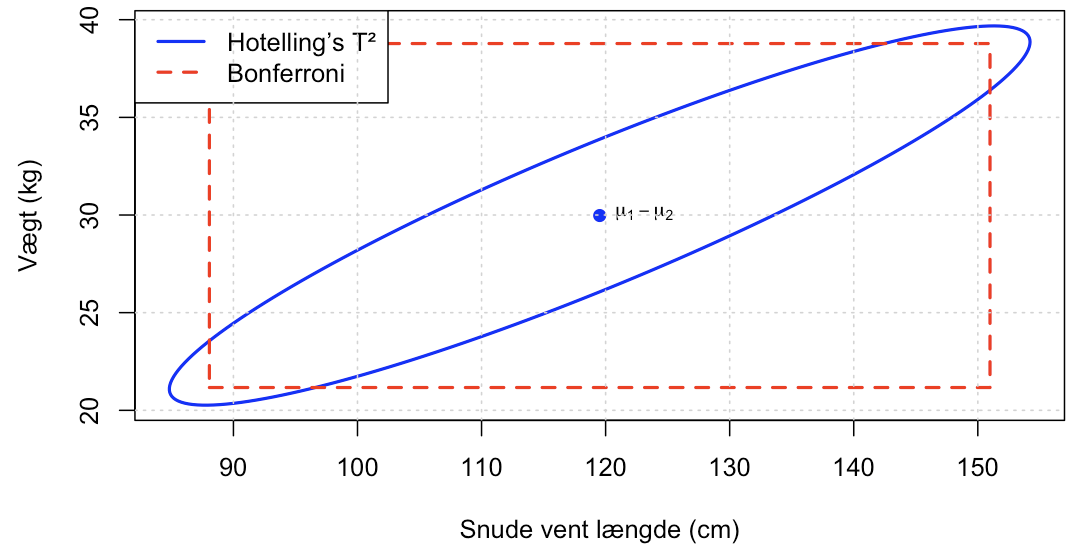
\includegraphics[height=0.5\linewidth]{plots/simultan6.png}
  		
		\textbf{\textcolor{junglegreen}{Figur 4:}} Simultane konfidensintervaller ikke indeholdende punktet (0,0)
		
	\end{figure}

\begin{center}
Snude vent længde (cm): \textcolor{blue}{[84.8 ; 154.2]}, \textcolor{red}{[88.1 ; 151.0]} \quad
Vægt (kg): \textcolor{blue}{[20.3 ; 39.7]}, \textcolor{red}{[21.2 ; 38.8]}
\end{center}



  \end{block}
  
  
  

  \vspace{-1em}   
  \begin{block}{Antagelser og resultater}
  \justifying

Resultaterne fra univariat- og multivariat- inferens kræver, at man kritisk forholder sig til de underliggende antagelser. \textbf{Univariat T-test bygger på antagelsen om marginal normalfordeling}, imens \textbf{Hotellings T2-test teoretisk forudsætter, at data følger en multivariat normalfordeling}. Manova og Box’s M-test antager, at \textbf{grupperne har ens kovariansstrukturer}. Normalitetsantagelsen er central, særligt i tolkningen af p-værdier fra tests som Box’s M, hvor teststørrelsen følger en chi-i-anden-fordeling under antagelse af normalitet. I vores analyser indikerer Q-Q plots dog, at \textbf{denne antagelse ikke er opfyldt} – hverken univariat eller multivariat. Derfor bør resultaterne tolkes med forsigtighed, da brud på disse forudsætninger kan påvirke testenes gyldighed og pålidelighed.

\end{block}
  


\vspace{-1em} 
\begin{block}{Konklusion}
  \justifying
	
\textbf{Der er signifikant forskel i både længde og vægt mellem han- og hun-anakondaer}. 

	\vspace{0.10em}

	
	De univariate og multivariate hypotesetest forkaster klart nulhypotesen om ens middelværdier. Hun-anakondaer er typisk både længere og tungere end hanner – et fænomen kendt som \textbf{omvendt kønsdimorfisme}, hvor hunnen er størst. Denne forskel spiller en vigtig rolle under parringsritualer, hvor flere hanner samles omkring en stor hun. I de simultane konfidensintervaller ligger punktet (0, 0) tydeligt udenfor, hvilket bekræfter forskellen mellem kønnene.

\end{block}


  	\vspace{-1em} 
  	\begin{figure}[h!]
		\centering
		
\includegraphics[width=1\linewidth]{plots/snake.png}
  		
		\textbf{\textcolor{junglegreen}{Figur 5:}} Illustration af anakondaens størrelser
	\end{figure}

\end{column}

\separatorcolumn
\end{columns}
\end{frame}

\end{document}
